% CS615 Aspects of System Administration
% Author: Jan Schaumann <jschauma@netmeister.org>
% $Id: slides.tex,v 1.3 2005/01/24 03:39:55 jschauma Exp $

\documentclass[xga]{xdvislides}
\usepackage[landscape]{geometry}
\usepackage{graphics}
\usepackage{graphicx}
\usepackage{colordvi}

\newcommand{\smallish}{\fontsize{18}{18}\selectfont}

\begin{document}
\setfontphv

%%% Headers and footers
\lhead{\slidetitle}				% default:\lhead{\slidetitle}
\chead{CS615 - Aspects of System Administration}% default:\chead{\relax}
\rhead{Slide \thepage}				% default:\rhead{\sectiontitle}
\lfoot{\Gray{Lecture 01: Introduction}}		% default:\lfoot{\slideauthor}
\cfoot{\relax}					% default:\cfoot{\relax}
\rfoot{\Gray{\today}}

\vspace*{\fill}
\begin{center}
	\Hugesize
		CS615 - Aspects of System Administration\\ [1em]
	\hspace*{5mm}\blueline\\ [1em]
	\Normalsize
		Department of Computer Science\\
		Stevens Institute of Technology\\
		Jan Schaumann\\
		\verb+jschauma@stevens.edu+ \\
		\verb+http://www.cs.stevens.edu/~jschauma/615/+
\end{center}
\vspace*{\fill}

\subsection{Why are you here?}

\vspace*{\fill}
\Hugesize
{\tt https://www.cs.stevens.edu/\~{}jschauma/cgi-bin/615.cgi}
\Normalsize
\vspace*{\fill}

\subsection{The Job of a System Administrator}
What {\bf exactly} does a {\em System Administrator} do?

\subsection{The Job of a System Administrator}
\begin{figure}[hb]
	\begin{center}
		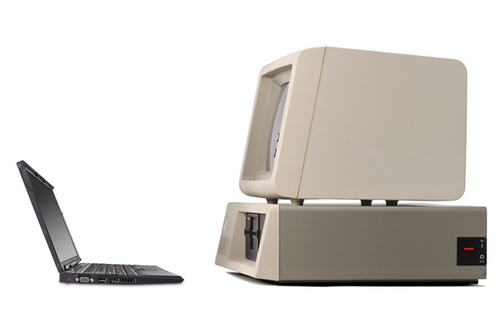
\includegraphics[scale=0.9]{pics/computers.eps} \\
	\end{center}
\end{figure}

\subsection{The Job of a System Administrator}
\vspace*{\fill}
\begin{figure}[hb]
	\begin{center}
		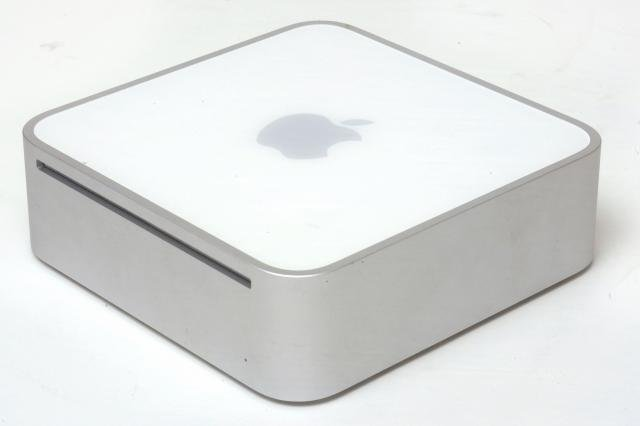
\includegraphics[scale=0.6]{pics/macmini.eps} \\
	\end{center}
\end{figure}
\vspace*{\fill}

\subsection{The Job of a System Administrator}
\vspace*{\fill}
\begin{figure}[hb]
	\begin{center}
		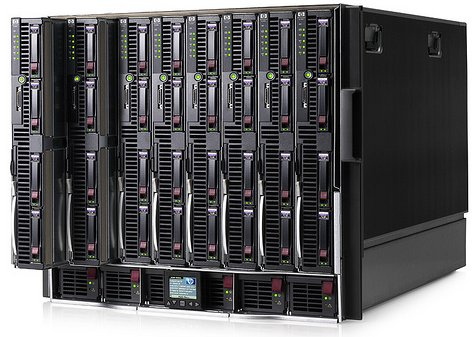
\includegraphics[scale=1.0]{pics/blades.eps} \\
	\end{center}
\end{figure}
\vspace*{\fill}

\subsection{The Job of a System Administrator}
\vspace*{\fill}
\begin{figure}[hb]
	\begin{center}
		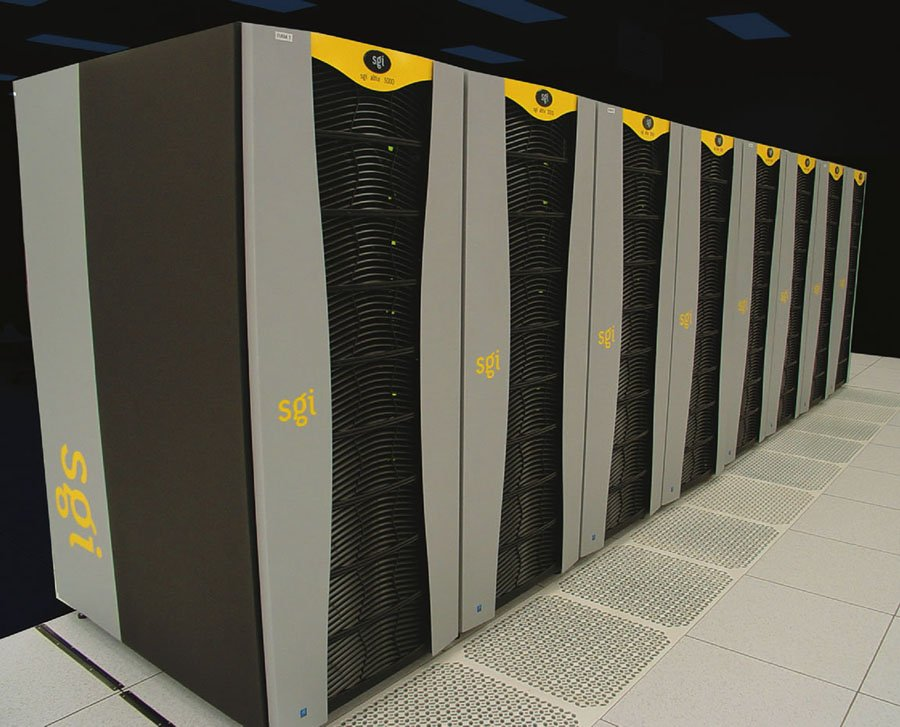
\includegraphics[scale=0.4]{pics/altix.eps} \\
	\end{center}
\end{figure}
\vspace*{\fill}

\subsection{The Job of a System Administrator}
\vspace*{\fill}
\begin{figure}[hb]
	\begin{center}
		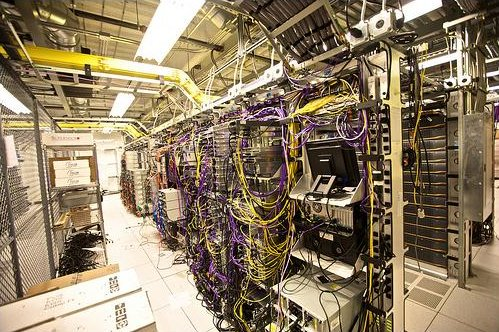
\includegraphics[scale=0.8]{pics/datacenter.eps} \\
	\end{center}
\end{figure}
\vspace*{\fill}

\subsection{The Job of a System Administrator}
\vspace*{\fill}
\begin{figure}[hb]
	\begin{center}
		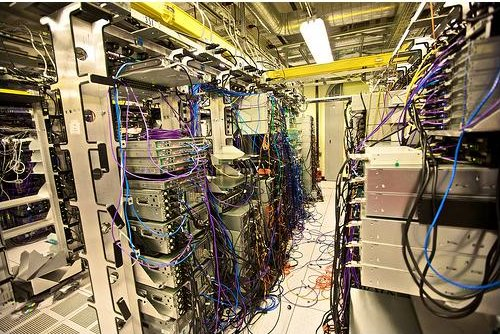
\includegraphics[scale=0.8]{pics/datacenter2.eps} \\
	\end{center}
\end{figure}
\vspace*{\fill}



\subsection{The Job of a System Administrator}
\vspace*{\fill}
\begin{figure}[hb]
	\begin{center}
		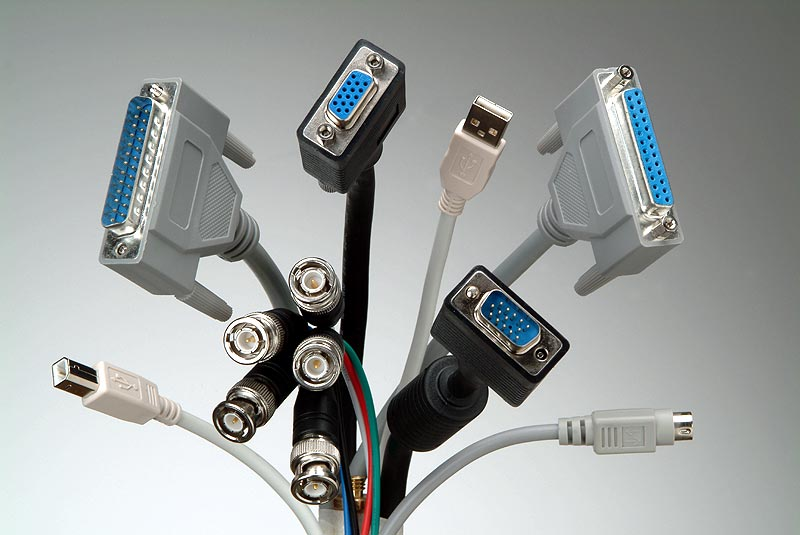
\includegraphics[scale=0.7]{pics/computer-cables-big.eps} \\
	\end{center}
\end{figure}
\vspace*{\fill}

\subsection{The Job of a System Administrator}
\vspace*{\fill}
\begin{figure}[hb]
	\begin{center}
		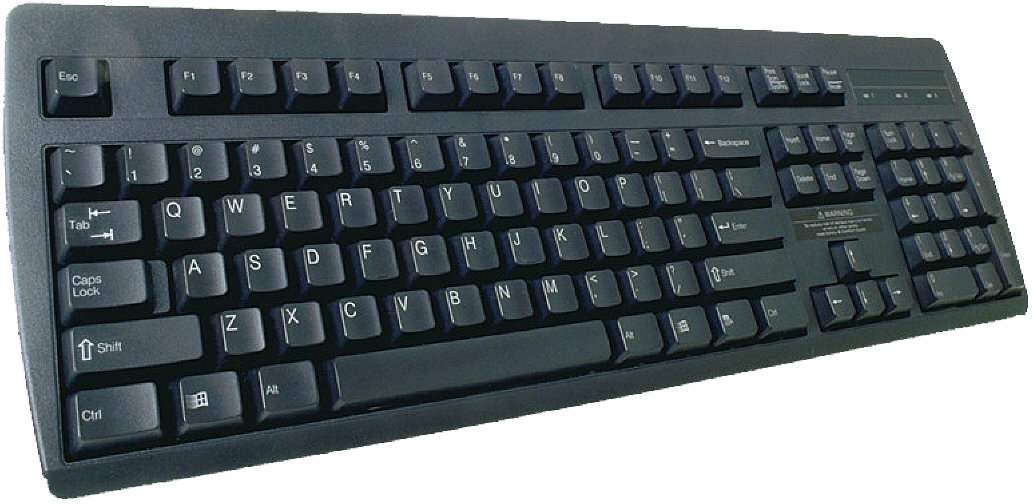
\includegraphics[scale=4.0]{pics/keyboard.eps} \\
	\end{center}
\end{figure}
\vspace*{\fill}

\subsection{The Job of a System Administrator}
\vspace*{\fill}
\begin{figure}[hb]
	\begin{center}
		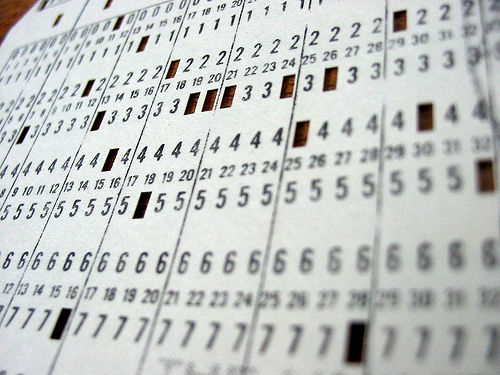
\includegraphics[scale=0.7]{pics/punchcard.eps} \\
	\end{center}
\end{figure}
\vspace*{\fill}

\subsection{The Job of a System Administrator}
\vspace*{\fill}
\begin{figure}[hb]
	\begin{center}
		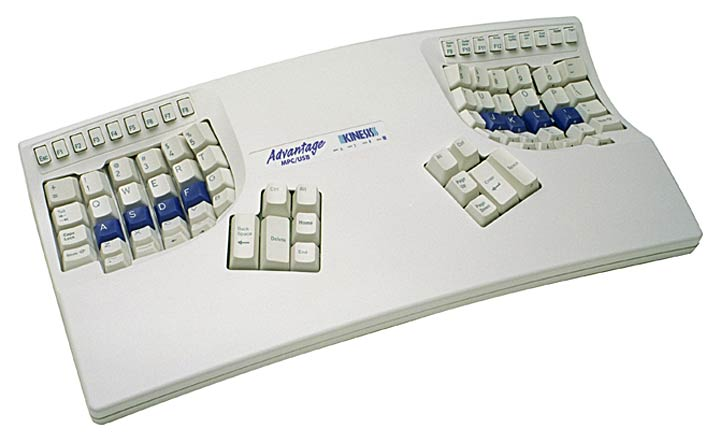
\includegraphics[scale=0.9]{pics/kinesis.eps} \\
	\end{center}
\end{figure}
\vspace*{\fill}

\subsection{The Job of a System Administrator}
\vspace*{\fill}
\begin{figure}[hb]
	\begin{center}
		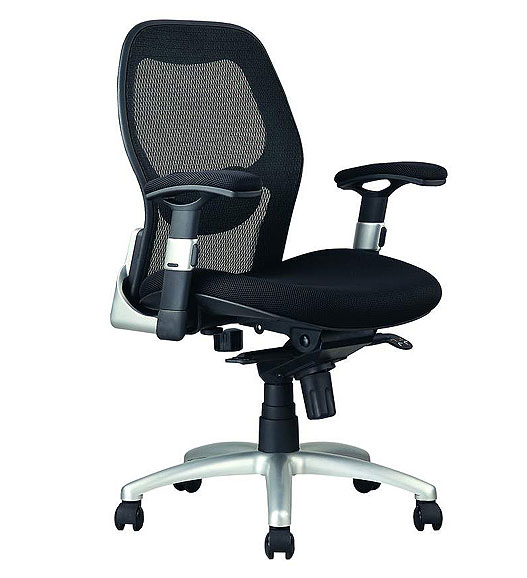
\includegraphics[scale=0.65]{pics/office-chair.eps} \\
	\end{center}
\end{figure}
\vspace*{\fill}

\subsection{The Job of a System Administrator}
\vspace*{\fill}
\begin{figure}[hb]
	\begin{center}
		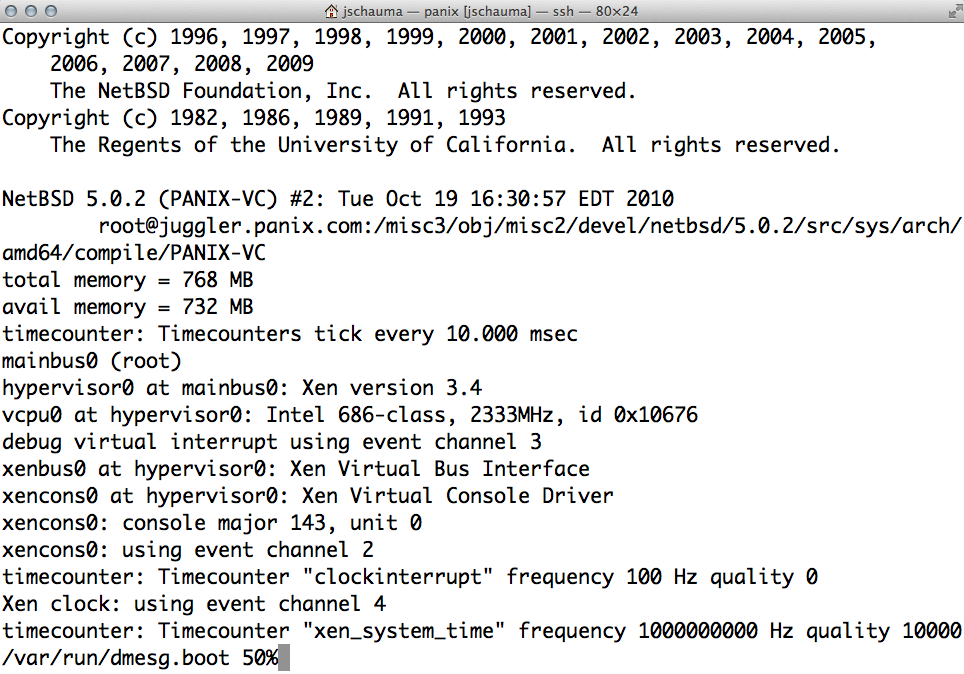
\includegraphics[scale=0.4]{pics/dmesg.eps} \\
	\end{center}
\end{figure}
\vspace*{\fill}

\subsection{The Job of a System Administrator}
\vspace*{\fill}
\begin{figure}[hb]
	\begin{center}
		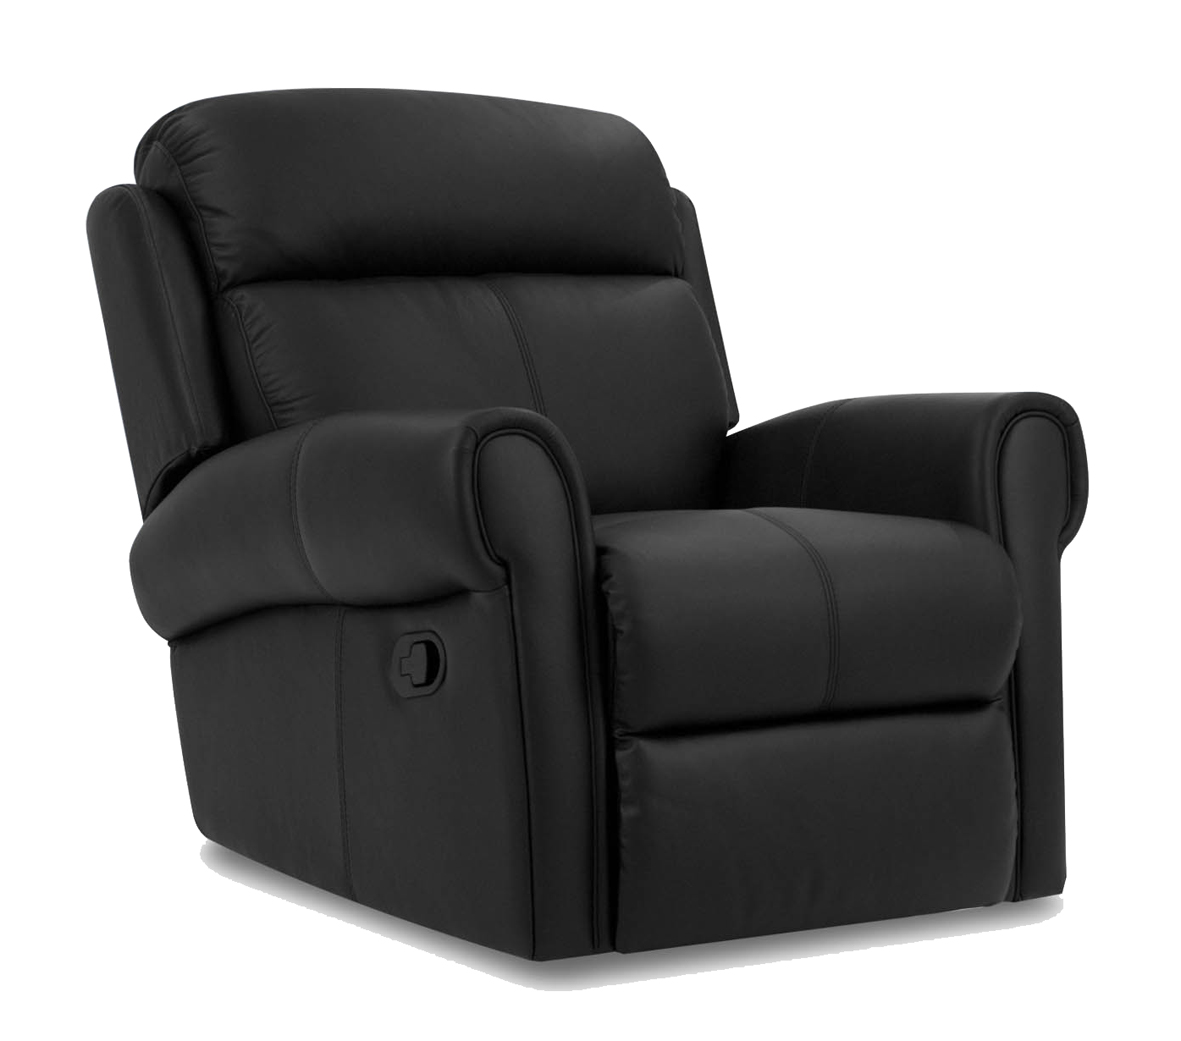
\includegraphics[scale=1.1]{pics/armchair.eps} \\
	\end{center}
\end{figure}
\vspace*{\fill}

\subsection{The Job of a System Administrator}
\vspace*{\fill}
\begin{figure}[hb]
	\begin{center}
		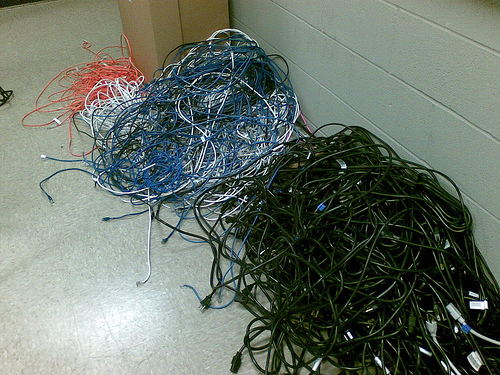
\includegraphics[scale=0.7]{pics/cable-mess.eps} \\
	\end{center}
\end{figure}
\vspace*{\fill}

\subsection{The Job of a System Administrator}
\vspace*{\fill}
\begin{figure}[hb]
	\begin{center}
		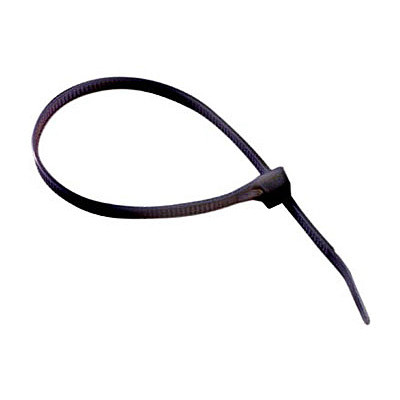
\includegraphics[scale=0.7]{pics/Cable_Tie.eps} \\
	\end{center}
\end{figure}
\vspace*{\fill}

\subsection{The Job of a System Administrator}
\vspace*{\fill}
\begin{figure}[hb]
	\begin{center}
		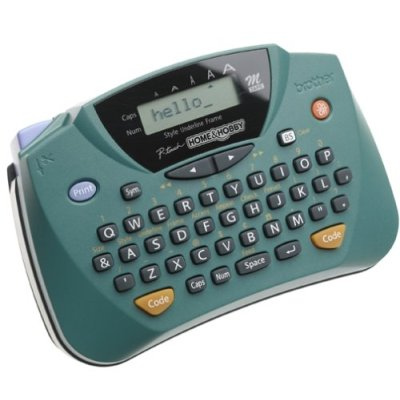
\includegraphics[scale=0.7]{pics/labelmaker.eps} \\
	\end{center}
\end{figure}
\vspace*{\fill}

\subsection{The Job of a System Administrator}
\vspace*{\fill}
\begin{figure}[hb]
	\begin{center}
		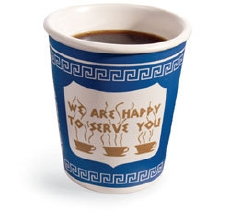
\includegraphics[scale=1.2]{pics/coffee.eps} \\
	\end{center}
\end{figure}
\vspace*{\fill}

\subsection{The Job of a System Administrator}
\vspace*{\fill}
\begin{figure}[hb]
	\begin{center}
		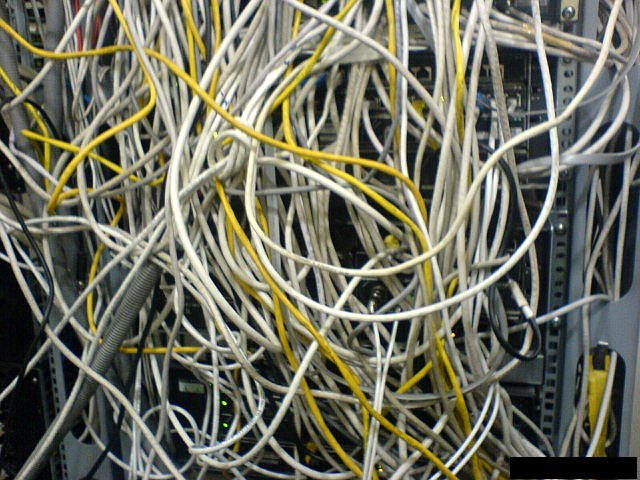
\includegraphics[scale=0.6]{pics/cable_mess.eps} \\
	\end{center}
\end{figure}
\vspace*{\fill}

\subsection{The Job of a System Administrator}
\vspace*{\fill}
\begin{figure}[hb]
	\begin{center}
		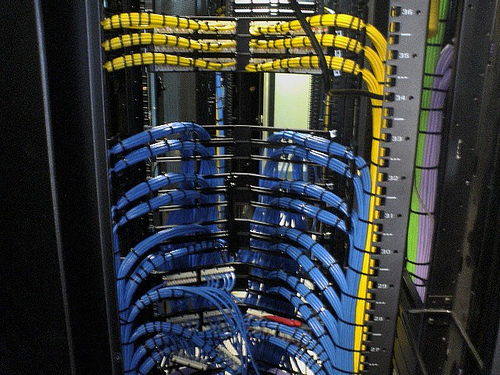
\includegraphics[scale=0.7]{pics/cables2.eps} \\
	\end{center}
\end{figure}
\vspace*{\fill}

\subsection{The Job of a System Administrator}
\vspace*{\fill}
\begin{figure}[hb]
	\begin{center}
		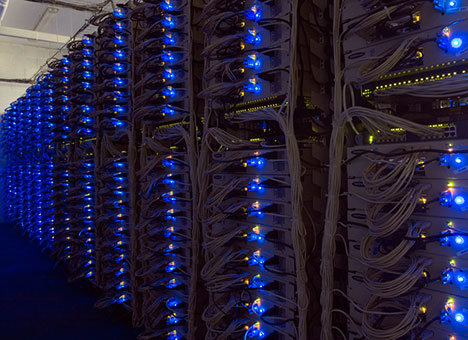
\includegraphics[scale=1.1]{pics/data-center-servers-t001.eps} \\
	\end{center}
\end{figure}
\vspace*{\fill}

\subsection{The Job of a System Administrator}
\vspace*{\fill}
\begin{figure}[hb]
	\begin{center}
		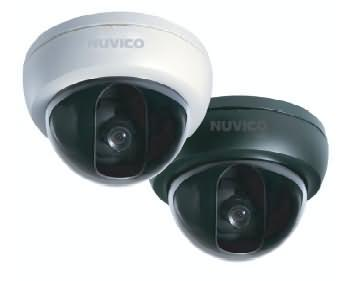
\includegraphics[scale=0.9]{pics/camera.eps} \\
	\end{center}
\end{figure}
\vspace*{\fill}

\subsection{The Job of a System Administrator}
\vspace*{\fill}
\begin{figure}[hb]
	\begin{center}
		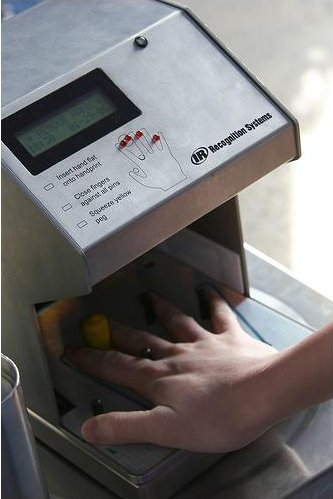
\includegraphics[scale=0.5]{pics/hand-scanner.eps} \\
	\end{center}
\end{figure}
\vspace*{\fill}


\subsection{The Job of a System Administrator}
\vspace*{\fill}
\begin{center}
	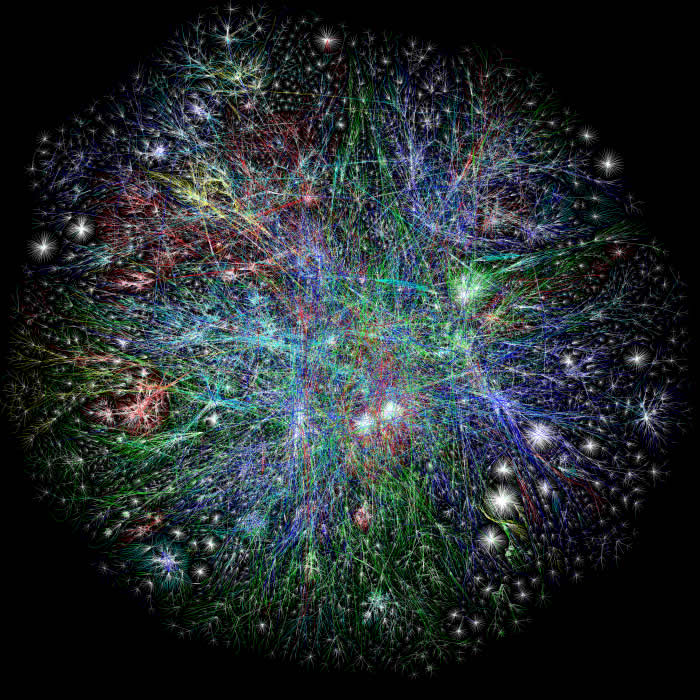
\includegraphics[scale=0.3]{pics/internet.eps} \\
	\small
	{\tt http://www.opte.org/maps/}
	\Normalsize
\end{center}
\vspace*{\fill}

\subsection{The Job of a System Administrator}
\vspace*{\fill}
\begin{figure}[hb]
	\begin{center}
		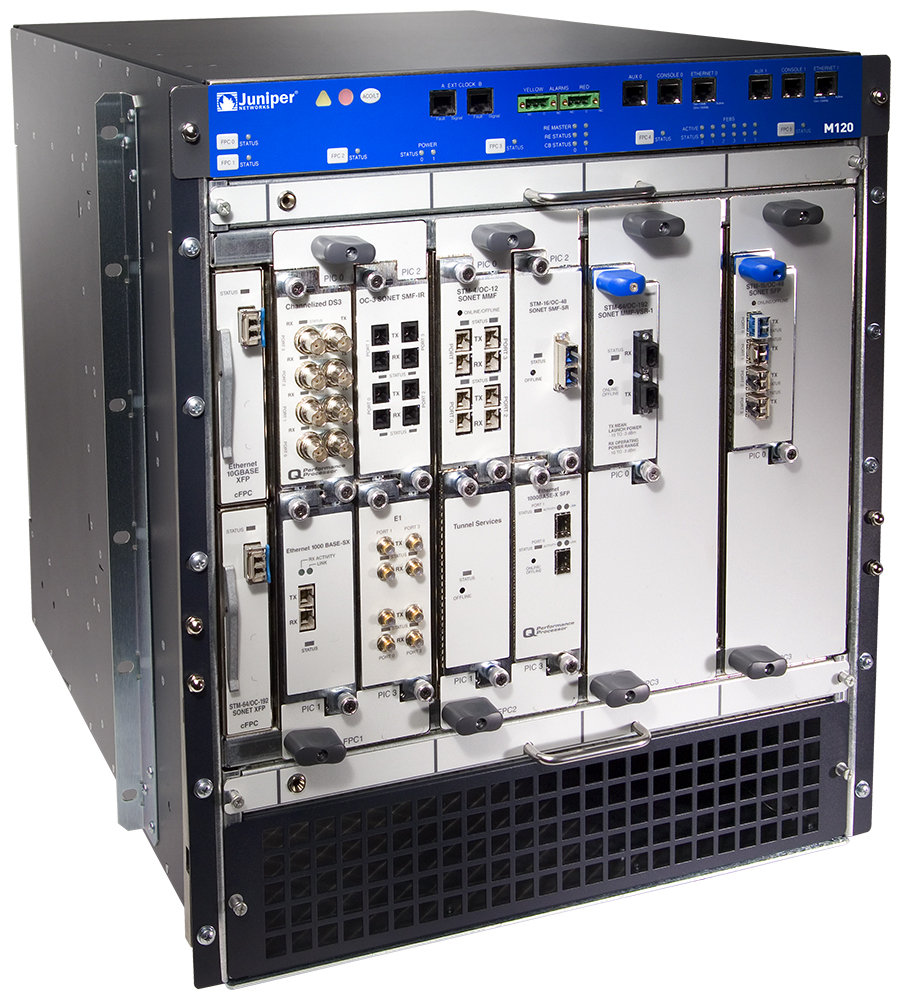
\includegraphics[scale=0.4]{pics/juniper.eps} \\
	\end{center}
\end{figure}
\vspace*{\fill}

\subsection{The Job of a System Administrator}
\vspace*{\fill}
\begin{figure}[hb]
	\begin{center}
		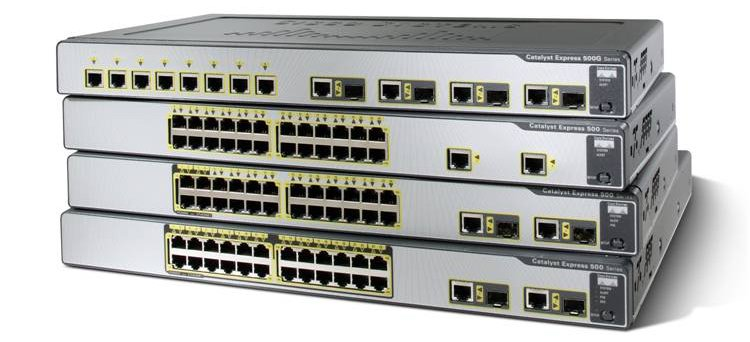
\includegraphics[scale=1.6]{pics/switches.eps} \\
	\end{center}
\end{figure}
\vspace*{\fill}

\subsection{The Job of a System Administrator}
\vspace*{\fill}
\begin{figure}[hb]
	\begin{center}
		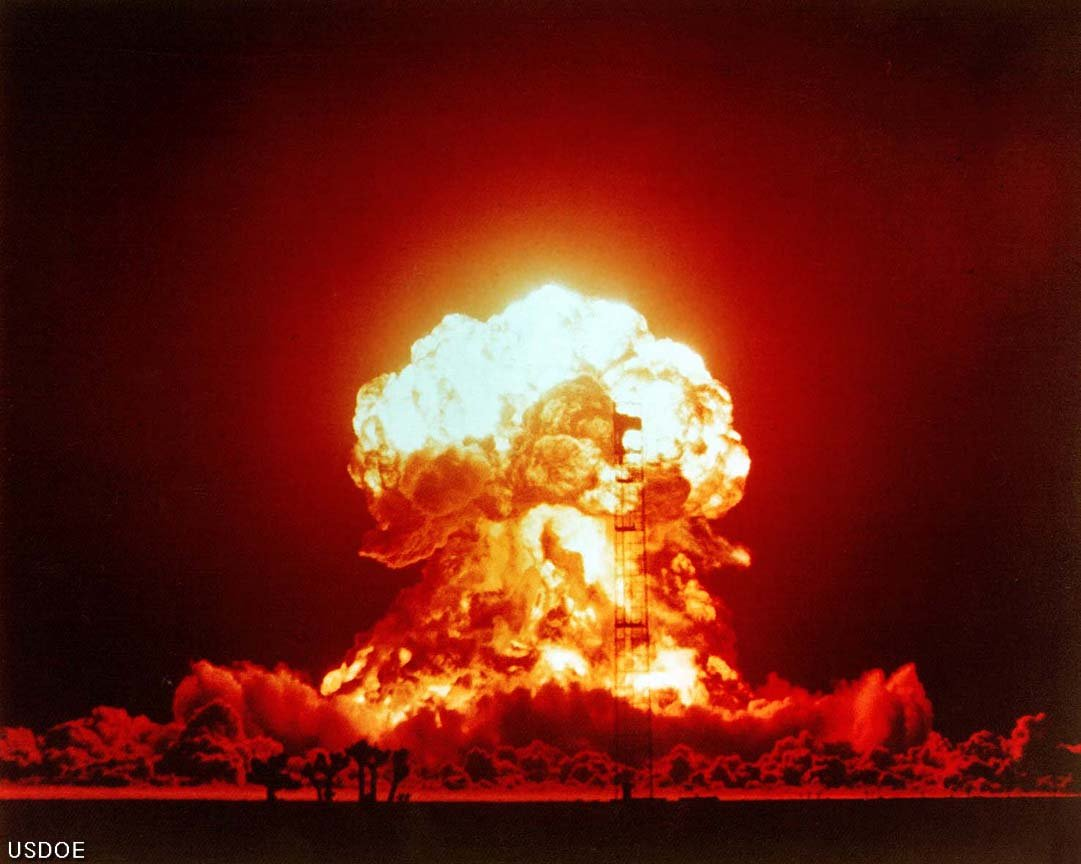
\includegraphics[scale=0.3]{pics/mushroom_cloud.eps} \\
	\end{center}
\end{figure}
\vspace*{\fill}

\subsection{The Job of a System Administrator}
\vspace*{\fill}
\begin{figure}[hb]
	\begin{center}
		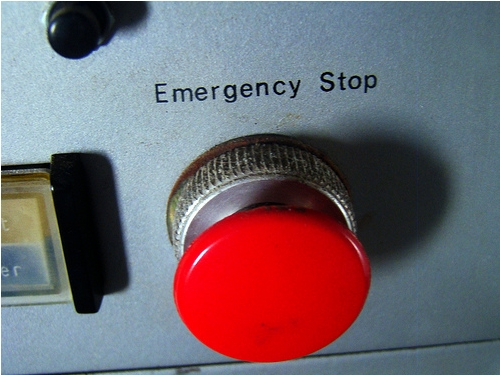
\includegraphics[scale=0.75]{pics/big-red-button.eps} \\
	\end{center}
\end{figure}
\vspace*{\fill}

\subsection{The Job of a System Administrator}
\vspace*{\fill}
\begin{figure}[hb]
	\begin{center}
		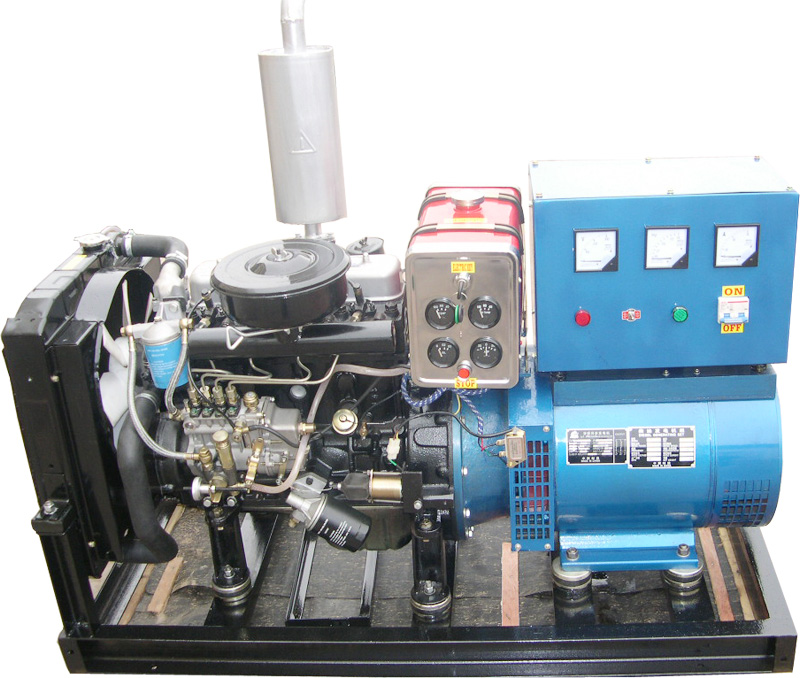
\includegraphics[scale=1.8]{pics/diesel-generator.eps} \\
	\end{center}
\end{figure}
\vspace*{\fill}

\subsection{The Job of a System Administrator}
\vspace*{\fill}
\begin{figure}[hb]
	\begin{center}
		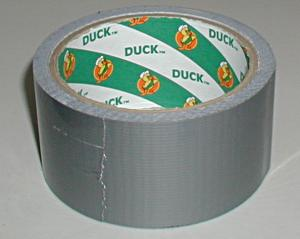
\includegraphics[scale=1.0]{pics/DuckTape.eps} \\
	\end{center}
\end{figure}
\vspace*{\fill}

\subsection{The Job of a System Administrator}
\vspace*{\fill}
\begin{figure}[hb]
	\begin{center}
		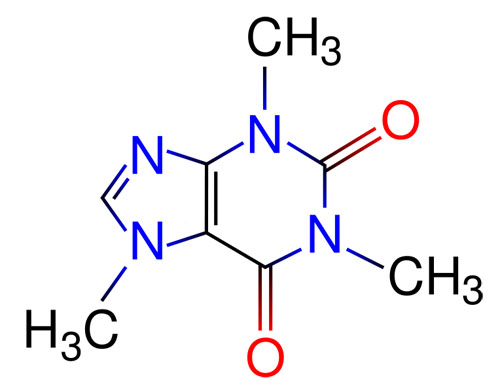
\includegraphics[scale=0.65]{pics/Caffeine_molecule.eps} \\
	\end{center}
\end{figure}
\vspace*{\fill}

\subsection{The Job of a System Administrator}
\vspace*{\fill}
\begin{figure}[hb]
	\begin{center}
		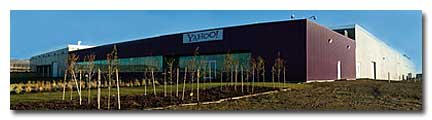
\includegraphics[scale=2.0]{pics/quincy-panorama.eps} \\
	\end{center}
\end{figure}
\vspace*{\fill}

\subsection{The Job of a System Administrator}
\vspace*{\fill}
\begin{figure}[hb]
	\begin{center}
		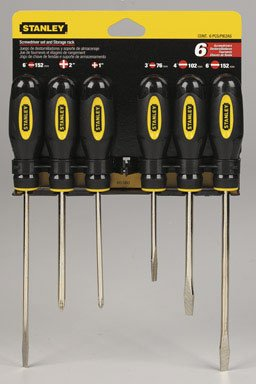
\includegraphics[scale=0.75]{pics/screwdrivers.eps} \\
	\end{center}
\end{figure}
\vspace*{\fill}

\subsection{The Job of a System Administrator}
\vspace*{\fill}
\begin{figure}[hb]
	\begin{center}
		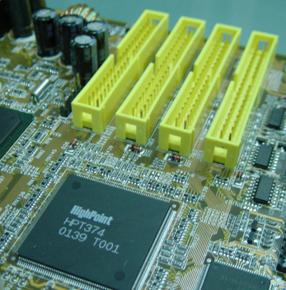
\includegraphics[scale=1.2]{pics/raid.eps} \\
	\end{center}
\end{figure}
\vspace*{\fill}

\subsection{The Job of a System Administrator}
\vspace*{\fill}
\begin{figure}[hb]
	\begin{center}
		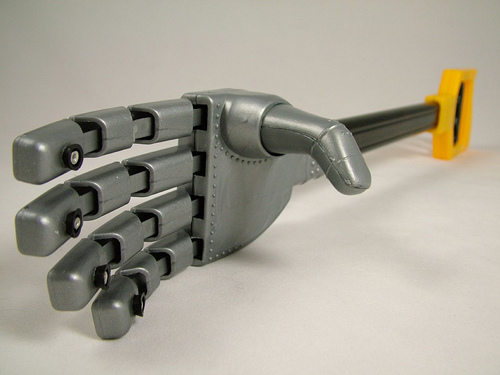
\includegraphics[scale=0.7]{pics/remote_hands.eps} \\
	\end{center}
\end{figure}
\vspace*{\fill}

\subsection{The Job of a System Administrator}
\vspace*{\fill}
\begin{figure}[hb]
	\begin{center}
		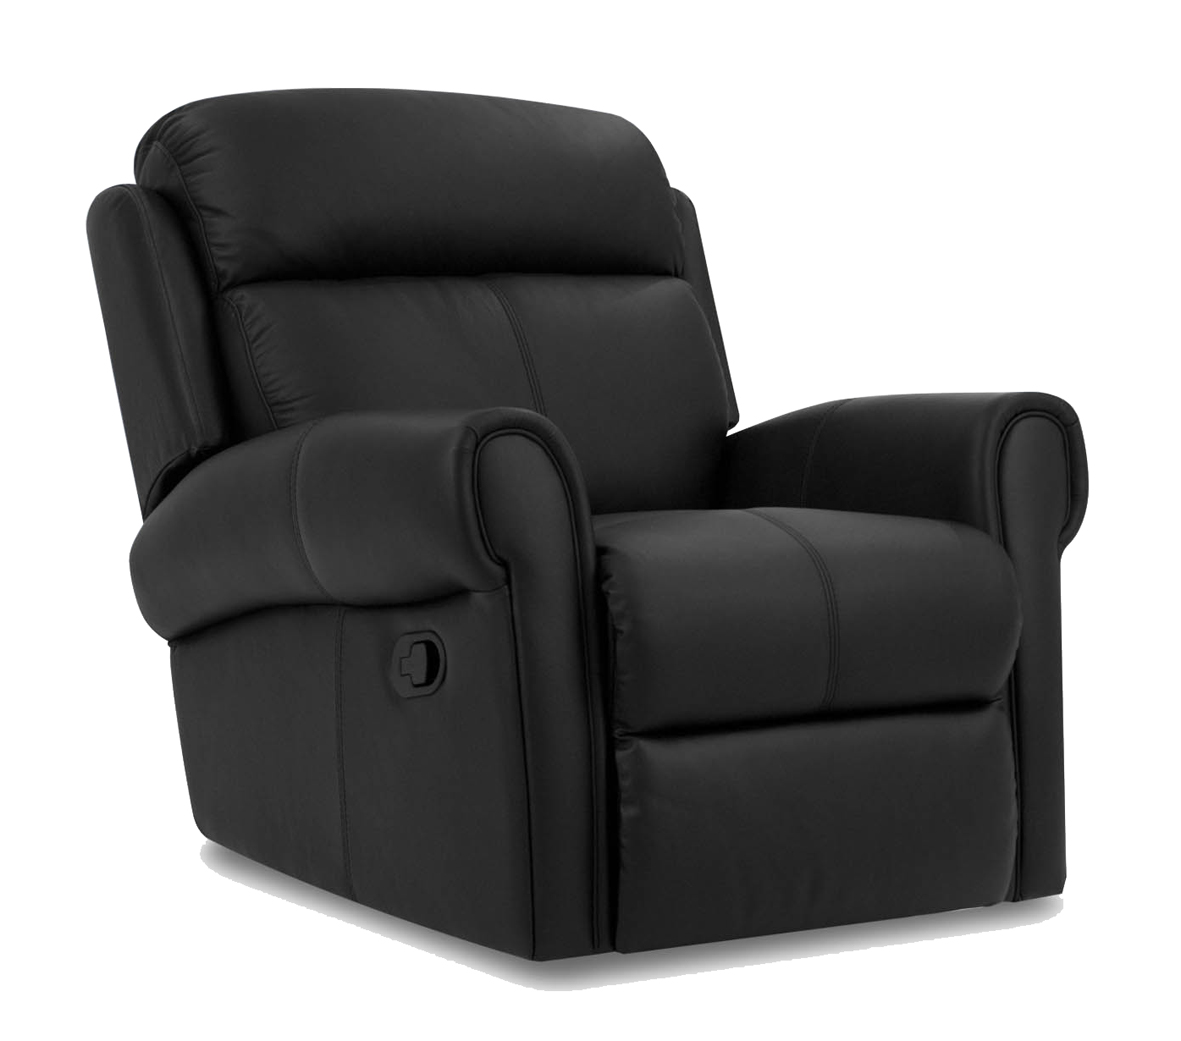
\includegraphics[scale=1.1]{pics/armchair.eps} \\
	\end{center}
\end{figure}
\vspace*{\fill}

\subsection{The Job of a System Administrator}
\vspace*{\fill}
\begin{figure}[hb]
	\begin{center}
		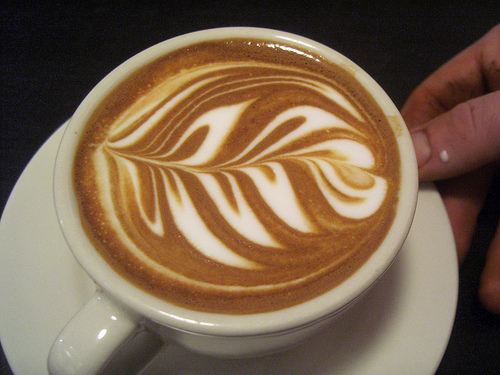
\includegraphics[scale=0.75]{pics/cappuccino.eps} \\
	\end{center}
\end{figure}
\vspace*{\fill}

\subsection{The Job of a System Administrator}
\vspace*{\fill}
\begin{figure}[hb]
	\begin{center}
		
\includegraphics[scale=0.8]{pics/spam.eps} \\
	\end{center}
\end{figure}
\vspace*{\fill}

\subsection{The Job of a System Administrator}
\vspace*{\fill}
\begin{figure}[hb]
	\begin{center}
		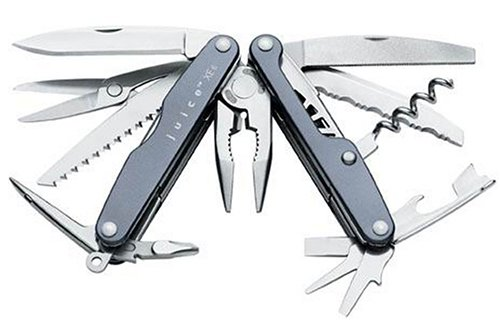
\includegraphics[scale=0.85]{pics/leatherman.eps} \\
	\end{center}
\end{figure}
\vspace*{\fill}

\subsection{The Job of a System Administrator}
\vspace*{\fill}
\begin{figure}[hb]
	\begin{center}
		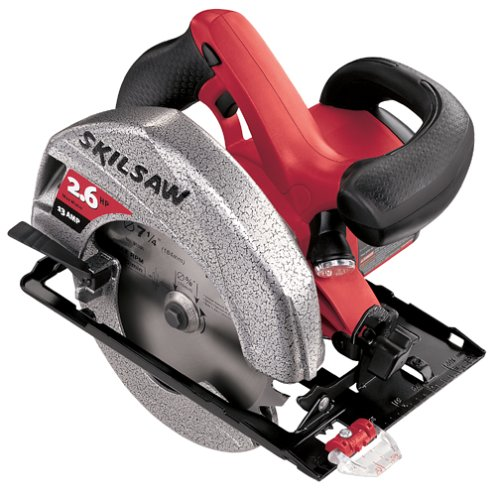
\includegraphics[scale=0.5]{pics/circularsaw.eps} \\
		\small See also: {\tt http://is.gd/WUezLL} \Normalsize
	\end{center}
\end{figure}
\vspace*{\fill}

\subsection{The Job of a System Administrator}
\vspace*{\fill}
\begin{figure}[hb]
	\begin{center}
		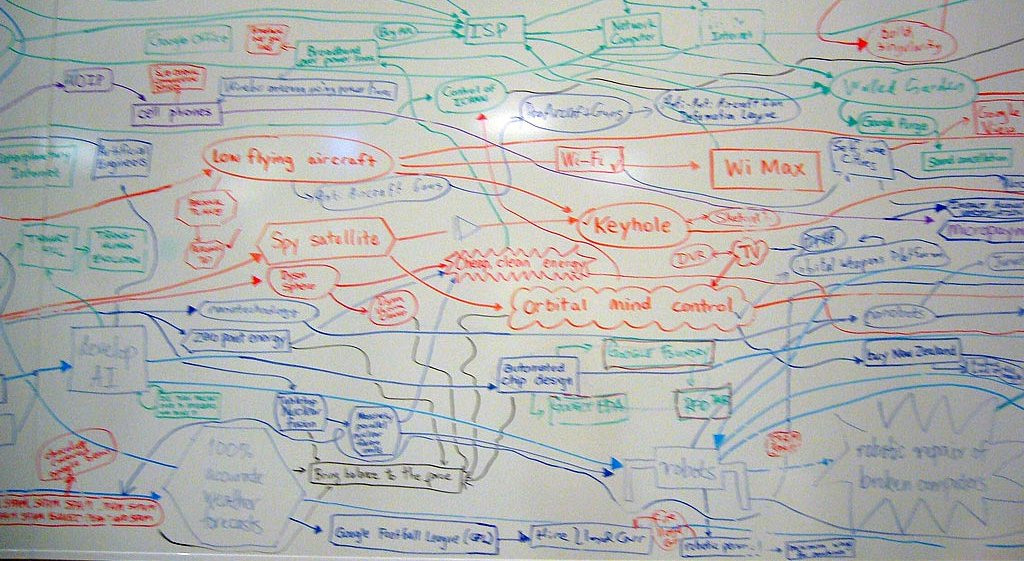
\includegraphics[scale=0.52]{pics/google_whiteboard_large.eps} \\
	\end{center}
\end{figure}
\vspace*{\fill}

\subsection{The Job of a System Administrator}
\vspace*{\fill}
\begin{figure}[hb]
	\begin{center}
		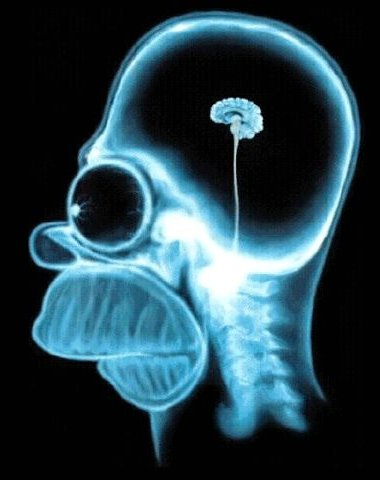
\includegraphics[scale=0.6]{pics/home-brain.eps} \\
	\end{center}
\end{figure}
\vspace*{\fill}

\subsection{The Job of a System Administrator}
What {\bf exactly} does a {\em System Administrator} do?

\subsection{The Job of a System Administrator}
What {\bf exactly} does a {\em System Administrator} do?
\begin{itemize}
	\item no precise job description
\end{itemize}

\subsection{The Job of a System Administrator}
What {\bf exactly} does a {\em System Administrator} do?
\begin{itemize}
	\item no precise job description
\end{itemize}
\begin{figure}[hb]
	\begin{center}
		
\includegraphics[scale=1.0]{pics/matrix.eps} \\
	\end{center}
\end{figure}



\subsection{The Job of a System Administrator}
What {\bf exactly} does a {\em System Administrator} do?
\begin{itemize}
	\item no precise job description
\end{itemize}
\vfill
 system administrator n.: \\
{\em one who, as a primary job function,
	manages computer and network systems on behalf of another, such as an
	employer or client.}

\subsection{The Job of a System Administrator}
What {\bf exactly} does a {\em System Administrator} do?
\begin{itemize}
	\item no precise job description
	\item often learned by experience
\end{itemize}
\vfill
system administrator n.: \\
{\em one who, as a primary job function,
	manages computer and network systems on behalf of another, such as an
	employer or client.}

\subsection{The Job of a System Administrator}
What {\bf exactly} does a {\em System Administrator} do?
\begin{itemize}
	\item no precise job description
	\item often learned by experience
	\item ``makes things run''
\end{itemize}
\vfill
system administrator n.: \\
{\em one who, as a primary job function,
	manages computer and network systems on behalf of another, such as an
	employer or client.}

\subsection{The Job of a System Administrator}
What {\bf exactly} does a {\em System Administrator} do?
\begin{itemize}
	\item no precise job description
	\item often learned by experience
	\item ``makes things run''
	\item work behind the scenes
\end{itemize}
\vfill
system administrator n.: \\
{\em one who, as a primary job function,
	manages computer and network systems on behalf of another, such as an
	employer or client.}

\subsection{The Job of a System Administrator}
What {\bf exactly} does a {\em System Administrator} do?
\begin{itemize}
	\item no precise job description
	\item often learned by experience
	\item ``makes things run''
	\item work behind the scenes
	\item often known as Operator, Network Administrator, System Programmer, System
		Manager, Service Engineer, Site Reliability Engineer etc.
\end{itemize}
\vfill
system administrator n.: \\
{\em one who, as a primary job function,
	manages computer and network systems on behalf of another, such as an
	employer or client.}

\subsection{So what is a {\em System}?}
``A group of interacting, interrelated, or interdependent elements that
together form a complex whole.''


\subsection{So what is a {\em System}?}
``A group of interacting, interrelated, or interdependent elements that
together form a complex whole.''
\\

In the context of this class, we generally consider {\em computer-human
systems} consisting of

\begin{itemize}
	\item the computer(s)
\end{itemize}

\subsection{So what is a {\em System}?}
``A group of interacting, interrelated, or interdependent elements that
together form a complex whole.''
\\

In the context of this class, we generally consider {\em computer-human
systems} consisting of

\begin{itemize}
	\item the computer(s)
	\item the network
\end{itemize}

\subsection{So what is a {\em System}?}
``A group of interacting, interrelated, or interdependent elements that
together form a complex whole.''
\\

In the context of this class, we generally consider {\em computer-human
systems} consisting of

\begin{itemize}
	\item the computer(s)
	\item the network
	\item the user(s)
\end{itemize}

\subsection{So what is a {\em System}?}
``A group of interacting, interrelated, or interdependent elements that
together form a complex whole.''
\\

In the context of this class, we generally consider {\em computer-human
systems} consisting of

\begin{itemize}
	\item the computer(s)
	\item the network
	\item the user(s)
	\item the organization's goals and policies
\end{itemize}

\subsection{... and {\em Administration}?}
Merriam Webster:
\begin{quote}
	{\bf administer, v:} {\em to manage or supervise the execution, use, or conduct of} \\
\end{quote}


\subsection{... and {\em Administration}?}
Merriam Webster:
\begin{quote}
	{\bf administer, v:} {\em to manage or supervise the execution, use, or conduct of} \\
\end{quote}

{\em System} Administration frequently also includes other tasks such as
\begin{itemize}
	\item system design and architecture
\end{itemize}

\subsection{... and {\em Administration}?}
Merriam Webster:
\begin{quote}
	{\bf administer, v:} {\em to manage or supervise the execution, use, or conduct of} \\
\end{quote}

{\em System} Administration frequently also includes other tasks such as
\begin{itemize}
	\item system design and architecture
	\item reliability studies
\end{itemize}

\subsection{... and {\em Administration}?}
Merriam Webster:
\begin{quote}
	{\bf administer, v:} {\em to manage or supervise the execution, use, or conduct of} \\
\end{quote}


{\em System} Administration frequently also includes other tasks such as
\begin{itemize}
	\item system design and architecture
	\item reliability studies
	\item resource management
\end{itemize}

\subsection{... and {\em Administration}?}
Merriam Webster:
\begin{quote}
	{\bf administer, v:} {\em to manage or supervise the execution, use, or conduct of} \\
\end{quote}

{\em System} Administration frequently also includes other tasks such as
\begin{itemize}
	\item system design and architecture
	\item reliability studies
	\item resource management
	\item system fault diagnosis
\end{itemize}

\subsection{... and {\em Administration}?} Merriam Webster: \begin{quote} {\bf
administer, v:} {\em to manage or supervise the execution, use, or conduct of}
\\ \end{quote}

{\em System} Administration frequently also includes other tasks such as
\begin{itemize}
	\item system design and architecture
	\item reliability studies
	\item resource management
	\item system fault diagnosis
	\item ...
\end{itemize}


\subsection{... and {\em Administration}?}
Merriam Webster:
\begin{quote}
	{\bf administer, v:} {\em to manage or supervise the execution, use, or conduct of} \\
\end{quote}

{\em System} Administration frequently also includes other tasks such as
\begin{itemize}
	\item system design and architecture
	\item reliability studies
	\item resource management
	\item system fault diagnosis
	\item ...
\end{itemize}
\vspace{.5in}

...all of which my involve a fair amount of {\em software development}, {\em
programming} and {\em scripting}.

\subsection{Learning System Administration}
System Administration is a profession with no fixed career path.

\subsection{Learning System Administration}
System Administration is a profession with no fixed career path.

\begin{itemize}
	\item few degree granting programs
\end{itemize}

\subsection{Learning System Administration}
System Administration is a profession with no fixed career path.

\begin{itemize}
	\item few degree granting programs
	\item heavy reliance on practical experience
\end{itemize}

\subsection{Learning System Administration}
System Administration is a profession with no fixed career path.

\begin{itemize}
	\item few degree granting programs
	\item heavy reliance on practical experience
	\item specializations in many different areas possible
\end{itemize}

\subsection{Learning System Administration}
System Administration is a profession with no fixed career path.

\begin{itemize}
	\item few degree granting programs
	\item heavy reliance on practical experience
	\item specializations in many different areas possible
	\item breadth of expertise as necessary as depth in some areas
\end{itemize}


\subsection{Learning System Administration}
System Administration is a profession with no fixed career path.

\begin{itemize}
	\item few degree granting programs
	\item heavy reliance on practical experience
	\item specializations in many different areas possible
	\item breadth of expertise as necessary as depth in some areas
	\item background knowledge and requirements vary
\end{itemize}

\subsection{Learning System Administration}
\vfill
\begin{center}
	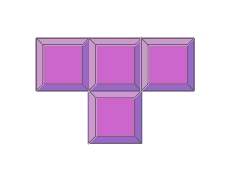
\includegraphics[scale=1.0]{pics/t.eps}
\end{center}
\vfill

\subsection{Learning System Administration}

Breadth of knowledge:
\begin{itemize}
	\item operating system concepts
	\item TCP/IP networking
	\item programming
	\item ...
\end{itemize}
\vspace{.5in}

Depth of knowledge:
\begin{itemize}
	\item certain OS flavor
	\item specific service (DNS, E-Mail, Databases, Content-Delivery, ...)
	\item specific implementation/vendor (Oracle, Hadoop, Apache, Cisco, ...)
	\item specific are of expertise (security, storage, network, data center, ...)
	\item ...
\end{itemize}

\subsection{SysAdmins' favorite Laws}
\smallish
Ockham's Razor:
\begin{quote}
{\em ``Of two equivalent theories or explanations, all other things being
equal, the simpler one is to be preferred.''}
\end{quote}
\Normalsize

\subsection{SysAdmins' favorite Laws}
\smallish
Ockham's Razor:
\begin{quote}
{\em ``Of two equivalent theories or explanations, all other things being
equal, the simpler one is to be preferred.''}
\end{quote}

2nd Law of Thermodynamics:
\begin{quote}
{\em ``The entropy of an isolated system always increases with time.''}
\end{quote}
\Normalsize

\subsection{SysAdmins' favorite Laws}
\smallish
Ockham's Razor:
\begin{quote}
{\em ``Of two equivalent theories or explanations, all other things being
equal, the simpler one is to be preferred.''}
\end{quote}

2nd Law of Thermodynamics:
\begin{quote}
{\em ``The entropy of an isolated system always increases with time.''}
\end{quote}

Hanlon's Razor:
\begin{quote}
{\em ``Never attribute to malice that which can be adequately explained by
stupidity.''}
\end{quote}
\Normalsize

\subsection{SysAdmins' favorite Laws}
\smallish
Ockham's Razor:
\begin{quote}
{\em ``Of two equivalent theories or explanations, all other things being
equal, the simpler one is to be preferred.''}
\end{quote}

2nd Law of Thermodynamics:
\begin{quote}
{\em ``The entropy of an isolated system always increases with time.''}
\end{quote}

Hanlon's Razor:
\begin{quote}
{\em ``Never attribute to malice that which can be adequately explained by
stupidity.''}
\end{quote}

Pareto's Principle:
\begin{quote}
{\em ``80\% of consequences stem from 20\% of the causes.''}
\end{quote}
\Normalsize

\subsection{SysAdmins' favorite Laws}
\smallish
Ockham's Razor:
\begin{quote}
{\em ``Of two equivalent theories or explanations, all other things being
equal, the simpler one is to be preferred.''}
\end{quote}

2nd Law of Thermodynamics:
\begin{quote}
{\em ``The entropy of an isolated system always increases with time.''}
\end{quote}

Hanlon's Razor:
\begin{quote}
{\em ``Never attribute to malice that which can be adequately explained by
stupidity.''}
\end{quote}

Pareto's Principle:
\begin{quote}
{\em ``80\% of consequences stem from 20\% of the causes.''}
\end{quote}

Sturgeon's Law:
\begin{quote}
{\em ``90\% of everything is crud.''}
\end{quote}
\Normalsize

\subsection{SysAdmins' favorite Laws}
\smallish
Ockham's Razor:
\begin{quote}
{\em ``Of two equivalent theories or explanations, all other things being
equal, the simpler one is to be preferred.''}
\end{quote}

2nd Law of Thermodynamics:
\begin{quote}
{\em ``The entropy of an isolated system always increases with time.''}
\end{quote}

Hanlon's Razor:
\begin{quote}
{\em ``Never attribute to malice that which can be adequately explained by
stupidity.''}
\end{quote}

Pareto's Principle:
\begin{quote}
{\em ``80\% of consequences stem from 20\% of the causes.''}
\end{quote}

Sturgeon's Law:
\begin{quote}
{\em ``90\% of everything is crud.''}
\end{quote}

Murphy's Law:
\begin{quote}
{\em ``If it can happen, it will happen.''}
\end{quote}
\Normalsize


\subsection{SysAdmins' favorite Laws}
\smallish
Ockham's Razor:
\begin{quote}
{\em ``Of two equivalent theories or explanations, all other things being
equal, the simpler one is to be preferred.''}
\end{quote}

2nd Law of Thermodynamics:
\begin{quote}
{\em ``The entropy of an isolated system always increases with time.''}
\end{quote}

Hanlon's Razor:
\begin{quote}
{\em ``Never attribute to malice that which can be adequately explained by
stupidity.''}
\end{quote}

Pareto's Principle:
\begin{quote}
{\em ``80\% of consequences stem from 20\% of the causes.''}
\end{quote}

Sturgeon's Law:
\begin{quote}
{\em ``90\% of everything is crud.''}
\end{quote}

Murphy's Law:
\begin{quote}
{\em ``If it can happen, it will happen.''}
\end{quote}

Throw in some philosophy for good measure:
\begin{quote}
{\em Causality: For every effect, there must be a cause.}
\end{quote}
\Normalsize

\subsection{SysAdmins' favorite tool}
\begin{center}
	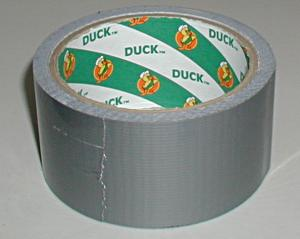
\includegraphics[scale=1.0]{pics/DuckTape.eps}
	% XXX include wd40-duck tape pic
\end{center}

\subsection{People think the internet looks like this.}
\begin{center}
	
\includegraphics[scale=0.7]{pics/cloud.eps}
\end{center}

\subsection{Or like this.}
\begin{center}
	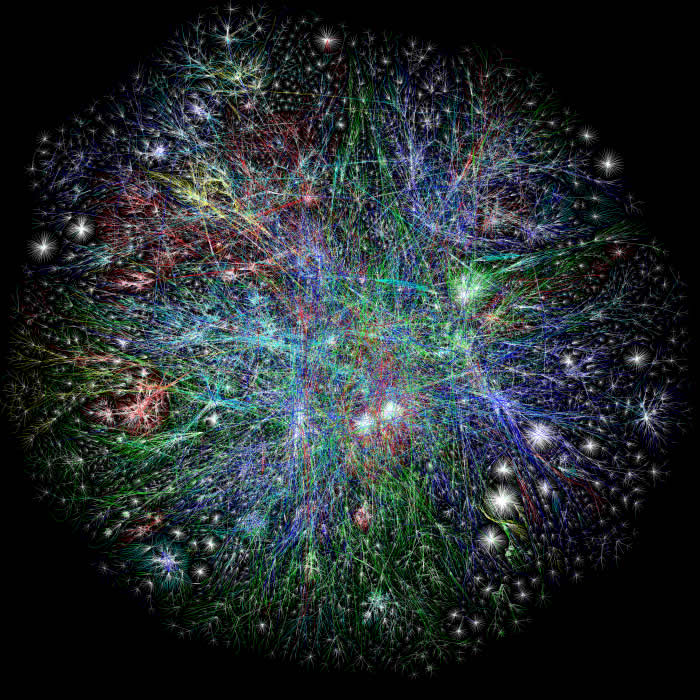
\includegraphics[scale=0.4]{pics/internet.eps}
\end{center}

\subsection{SysAdmins know it looks like this.}
\vspace*{\fill}
\begin{center}
    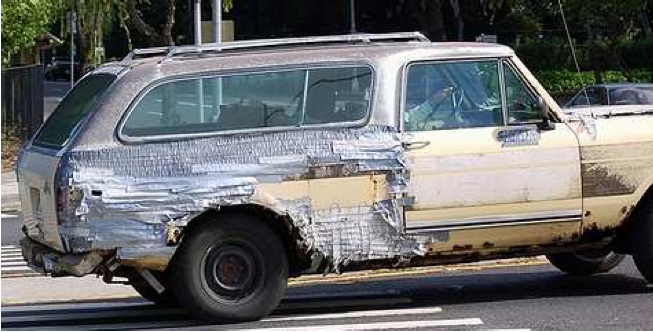
\includegraphics[scale=0.9]{pics/car-duct-tape.eps}
\end{center}
\vspace*{\fill}

\newpage
\vspace*{\fill}
\begin{center}
    \Hugesize
        Hooray! \\ [1em]
    \hspace*{5mm}
    \blueline\\
    \hspace*{5mm}\\
        5 Minute Break
\end{center}
\vspace*{\fill}

\subsection{In reality...}
\vspace*{\fill}
\begin{center}
    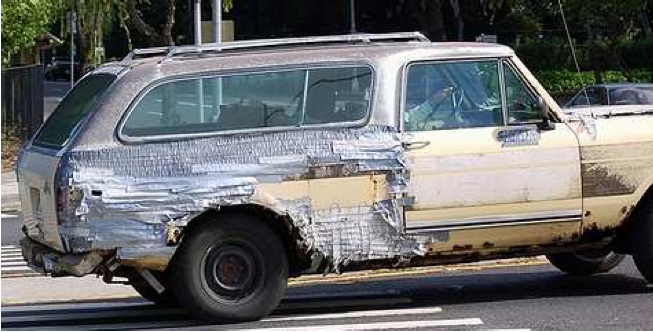
\includegraphics[scale=0.9]{pics/car-duct-tape.eps}
\end{center}
\vspace*{\fill}

\subsection{About this class}
We can only cover {\em some} of the aspects of System Administration.
\vspace*{\fill}
\begin{center}
	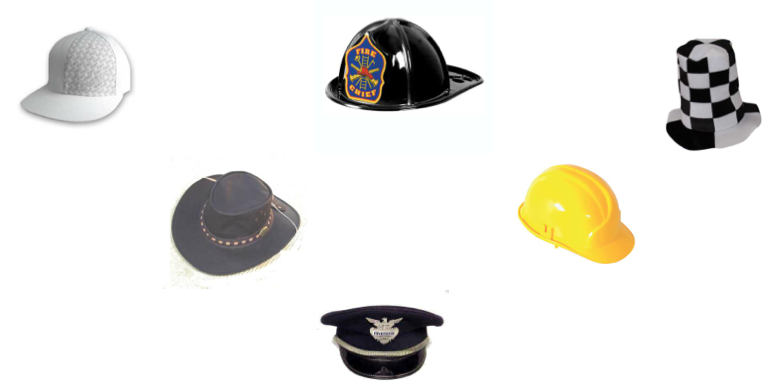
\includegraphics[scale=0.8]{pics/hats.eps}
\Normalsize
\end{center}
\vspace*{\fill}

\subsection{Three Pillars of Exceptional System Design}
We will give particular attention to these three core features:
\begin{itemize}
	\item Scalability
	\item Security
	\item Simplicity
\end{itemize}

\subsection{Three Pillars of Exceptional System Design: Scalability}
\vspace*{\fill}
\begin{center}
    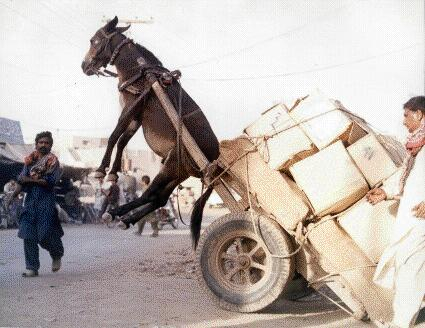
\includegraphics[scale=0.8]{pics/donkey_too_small_for_load.eps} \\
	System Overload
\end{center}
\vspace*{\fill}

\subsection{Three Pillars of Exceptional System Design: Scalability}
\vspace*{\fill}
\begin{center}
    \includegraphics[scale=0.2]{pics/donkey_too_small_for_load.eps} \\
    \includegraphics[scale=0.4]{pics/ardennes-horse.eps} \\
	Scaling Vertically
\end{center}
\vspace*{\fill}


\subsection{Three Pillars of Exceptional System Design: Scalability}
\vspace*{\fill}
\begin{center}
    \includegraphics[scale=0.2]{pics/donkey_too_small_for_load.eps} \\
    \includegraphics[scale=0.5]{pics/vierspaenner.eps} \\
	Scaling Horizontally
\end{center}
\vspace*{\fill}

\subsection{Three Pillars of Exceptional System Design: Scalability}
\vspace*{\fill}
\begin{center}
    \includegraphics[scale=0.2]{pics/donkey_too_small_for_load.eps} \\
    \includegraphics[scale=1.1]{pics/dogcart.eps} \\
	Scaling Down
\end{center}
\vspace*{\fill}

\subsection{Three Pillars of Exceptional System Design: Security}
\vspace*{\fill}
\begin{center}
    \includegraphics[scale=1.4]{pics/usability-security.eps} \\
\end{center}
\vspace*{\fill}

\subsection{Three Pillars of Exceptional System Design: Security}
\vspace*{\fill}
\begin{center}
    \includegraphics[scale=1.0]{pics/patch-bandaid.eps} \\
\end{center}
\vspace*{\fill}

\subsection{Three Pillars of Exceptional System Design: Security}
\vspace*{\fill}
\begin{center}
    \includegraphics[scale=1.4]{pics/wrong-usability.eps} \\
\end{center}
\vspace*{\fill}

\subsection{Three Pillars of Exceptional System Design: Security}
\vspace*{\fill}
\begin{center}
    \includegraphics[scale=1.1]{pics/better-usability.eps} \\
\end{center}
\vspace*{\fill}


\subsection{Three Pillars of Exceptional System Design: Simplicity}
\vspace*{\fill}
\begin{center}
    \includegraphics[scale=0.3]{pics/kiss.eps} \\
\end{center}
\vspace*{\fill}

\subsection{Three Pillars of Exceptional System Design: Simplicity}
\vspace*{\fill}
\begin{center}
    \includegraphics[scale=1.2]{pics/lego-block.eps} \\
\end{center}
\vspace*{\fill}

\subsection{Three Pillars of Exceptional System Design: Simplicity}
\vspace*{\fill}
\begin{center}
    \includegraphics[scale=0.1]{pics/millennium-falcon.eps} \\
\end{center}
\vspace*{\fill}







\subsection{About this class}
Suggested Reading:
\begin{itemize}
	\item ``Essential System Administration'', 3rd Edition, by \AE leen
		Frisch
	\item ``Unix System Administration Handbook'', 3rd Edition, by Evi Nemeth
	\item ``Principles of Network and System Administration'', by Mark Burgess
	\item ``Analytical Network and System Administration'', by Mark Burgess
	\item ``The Practice of System and Network Administration'', by Thomas
		A. Limoncelli \& Christine Hogan
\end{itemize}
\addvspace{.5in}
Grading:
\begin{itemize}
	\item class participation / lightning talks
	\item a number of homework assignments of varying weight
	\item a group project towards the end of the semester
	\item no curve
\end{itemize}

\subsection{Syllabus}
%Topics:
\begin{itemize}
	\item 2014-01-22: Introduction, Overview, course basics
	\item 2014-01-27: UNIX history and basics / Filesystems and Disks
	\item 2014-02-03: Software Installation Concepts
	\item 2014-02-10: User Management, multi-user basics
	\item 2014-02-18: Automating Administrative Tasks
	\item 2014-02-24: Backup and Disaster Recovery
	\item 2014-03-03: Networking
	\item 2014-03-17: Popular services (DNS, SMTP)
	\item 2014-03-24: Configuration Management (Guest Lecturer)
	\item 2014-03-31: Popular services (HTTP, SNMP, SSH)
	\item 2014-04-07: System Security
	\item 2014-04-14 -- 2011-04-28: AMA / Misc. topics / presentations / TBD
\end{itemize}

\subsection{Syllabus}
Miscellaneous topics and presentations may include:
\begin{itemize}
	\item large scale logging
	\item heterogenous networks / multiple OS
	\item automated installation
	\item configuration management
	\item server room basics, cooling issues, racking etc.
	\item clustering
	\item spam
	\item \ldots
\end{itemize}

\subsection{Questions, Answers, Chatter...}
\begin{itemize}
	\item 10 minutes of Ask Me Anything / current events / lightning talks at the beginning of the class \\
		\small that does {\em not} mean you can come 10 minutes late \Normalsize
	\\

	\item course website, syllabus, assignments, course material:\\
		\verb+https://www.cs.stevens.edu/~jschauma/615/+
	\\

	\item discussions and announcements:
		\verb+https://lists.stevens.edu/cgi-bin/mailman/listinfo/cs615asa+
	\\

	\item who knows what: \verb+https://twitter.com/cs615asa+
\end{itemize}

\subsection{Let's do some homework!}

{\tt https://webchat.freenode.net/ -- \#cs615asa} \\
\vspace{.25in}

{\tt http://www.cs.stevens.edu/~jschauma/615/s14-hw1.html} \\
\vspace{.25in}

\begin{itemize}
	\item ensure you have access to {\tt linux-lab.cs.stevens.edu}
	\item create your website (if you don't already have it)
	\item create an AWS account
	\item create an EC2 instance
	\item access EC2 instance, run commands
\end{itemize}

\subsection{Reading}
Miscellaneous:
\begin{itemize}
	\item \verb+http://www.opsschool.org/+
	\item \verb+http://nixsrv.com/llthw+
	\item \verb+http://linuxcommand.org/lc3_learning_the_shell.php+
	\item \verb+http://www.sage.org/pubs/22_jobs/+
\end{itemize}

UNIX history:
\begin{itemize}
	\item \verb+http://www.bell-labs.com/history/unix/+
	\item \verb+http://www.futuretech.blinkenlights.nl/admin/day1a.html+
	\item \verb+http://www.levenez.com/unix/+
	\item \verb+https://en.wikipedia.org/wiki/Operating_system+
\end{itemize}

\subsection{Reading}
UNIX basics:
\begin{itemize}
	\item chmod(1), chown(1), ls(1)
	\item intro(1), login(1), passwd(5)
	\item su(1), sudo(8)
\end{itemize}

%\nocite{*}
%\bibliographystyle{plain}
%\bibliography{slides}

\end{document}
